%Template for a pretty simple lab report @ HTW Berlin.
%This template is styled to compile with PDFLaTeX!

%start preamble
\documentclass[paper=a4,fontsize=11pt]{scrartcl}%kind of doc, font size, paper size
\usepackage[ngerman]{babel}%for special german letters etc			
\usepackage[T1]{fontenc}%same as t1enc but better						
\usepackage[utf8]{inputenc}%utf-8 encoding, other systems could use others encoding		
\usepackage{amsmath}%get math done
\usepackage{graphicx}%get pictures & graphics done
\graphicspath{{pictures/}}%folder to stash all kind of pictures etc
\usepackage[pdftex,hidelinks]{hyperref}%for links to web
\usepackage{amssymb}%symbolics for math
\usepackage{amsfonts}%extra fonts
\usepackage []{natbib}%citation style
\usepackage{caption}%captions under everything
\usepackage{listings}
\usepackage[titletoc]{appendix}
\numberwithin{equation}{section} 
\usepackage[printonlyused,withpage]{acronym}%how to handle acronyms
\usepackage{float}%for garphics and how to let them floating around in the doc
\usepackage{xcolor}%nicer colors, here used for links
\usepackage{wrapfig}%making graphics floated by text and not done by minipage
\usepackage{bashful}
\pdfpkresolution=2400%higher resolution

%settings colors for links
\hypersetup{
    colorlinks,
    linkcolor={blue!50!black},
    citecolor={blue},
    urlcolor={blue!80!black}
}

\lstdefinestyle{Bash}{
  language=bash,
  showstringspaces=false,
  basicstyle=\small\sffamily,
  numbers=left,
  numberstyle=\tiny,
  numbersep=5pt,
  frame=trlb,
  backgroundcolor=\color{gray!20},
  %linewidth=0.9\linewidth,
  %xleftmargin=0.5\linewidth
  %upquote=true,
  commentstyle=\color{red},
  keywordstyle=\color{blue},
  columns=fullflexible,
  literate={*}{{\char42}}1
         {-}{{\char45}}1
}


%%here begins the actual document%%

%%starts with title page%%
\begin{document}
\bibliographystyle{alpha}

\begin{titlepage}
%deckblatt start
\thispagestyle{empty}
\begin{center}

\includegraphics[width=0.45\textwidth]{HTW_Logo_rgb}\\
\end{center}
 
 
\begin{center}
\Large{Fachbereich 4 Wirtschaftswissenschaften II}
\end{center}
\begin{verbatim}
 
 
\end{verbatim}
\begin{center}
\textbf{\LARGE{Laborprotokoll}}\\
Netzwerke Übung\\
Sommersemester 2019
\end{center}
\begin{verbatim}
 

\end{verbatim}
\begin{center}
\textbf{im Studiengang Angewandte Informatik (B.Sc.)}
\end{center}
\begin{verbatim}
 
 
\end{verbatim}
 
\begin{flushleft}
\begin{tabular}{lllll}
\textbf{Thema:} & & Übungsblatt 02 -- Netzwerkgrundlagen \\
& & \texttt{Beispiellösung}\\
& & \\
& & \\
& & \\
\textbf{eingereicht von:}
& & Name1 \href{mailto: name1@htw-berlin.de}{name1@student.htw-berlin.de} & matrikel1\\
& & Name2 \href{mailto: name2@htw-berlin.de}{name2@student.htw-berlin.de} & matrikel2\\
& & Name3 \href{mailto: name3@htw-berlin.de}{name3@student.htw-berlin.de} & matrikel3\\
& & Name4 \href{mailto: name4@htw-berlin.de}{name4@student.htw-berlin.de} & matrikel4\\
\\
\textbf{eingereicht am:} & & \today\\
& & \\
& & \\
\end{tabular}
\end{flushleft}
\end{titlepage}

%starting TOC
\newpage
\tableofcontents
\newpage

\section{Einleitung}
Ziel des Laborprotokolls ist es Lösungswege aufzuzeigen, die es erlauben bestehende Netzwerkkonfigurationen zu analysieren und ein einfaches geswitchtes \ac{LAN} zu realisieren.
\subsection{Aufgaben- \& Problemstellung}
In der zweiten Laborübung haben wir uns erstmals mit der Konfiguration von Netzwerkadaptern auseinandergesetzt. Die dafür notwendigen Komponenten und das genutzte Betriebssystem werden im Abschnitt \ref{rpi} in Kürze beschrieben.\\

Zunächst untersuchen wir die Infrastruktur mithilfe des durch das \emph{\ac{DHCP}} vorkonfigurierten Netzwerkes. Dies repräsentiert den ersten Aufgabenteil und wird im Abschnitt \ref{conf_lan} beschrieben. Anschließend setzen wir ein eigenes statisches \emph{\ac{LAN}} um, das aus der Planung der Hausaufgaben hervorgeht. Die Protokollierung des geswitchten \emph{LAN}s ist im Abschnitt \ref{switched_lan} festgehalten.

\section{Hauptteil}
\subsection{Raspberry Pi} \label{rpi}
Die in der Laborübung genutzen Raspberry Pi 3 b+ sind sogenannte \acp{SoC}, die als vollständige Rechner gelten (\textit{Turing-vollständig}). Näheres zur Hardware kann unter \cite{rpi} gefunden werden.\\
Wir arbeiten auf einem \acs{GNU}/Linux System mit einer Raspbian Distribution (Debian-Fork) wie im Listing \ref{os-release} zu sehen ist.
\begin{lstlisting}[style=Bash, language=Bash, label=os-release]
cat /etc/os-release
NAME="Arch Linux"
PRETTY_NAME="Arch Linux"
ID=arch
ID_LIKE=archlinux
ANSI_COLOR="0;36"
HOME_URL="https://www.archlinux.org/"
SUPPORT_URL="https://bbs.archlinux.org/"
BUG_REPORT_URL="https://bugs.archlinux.org/"
\end{lstlisting}
\texttt{uname} gibt folgende Kernelspezifika aus:
\begin{lstlisting}[style=Bash, language=Bash]
uname -or
5.0.10-hardend-arch1-1-ARCH GNU/Linux # Linux Kernel 5.0.101 modifizierter, gehaerteten Kern
# RPI
uname -or
4.14.98-v7+ GNU/Linux
\end{lstlisting} 
Der Hostname alles Raspberry Pis lautet \emph{networkingLab}, auf diesen Rechnern arbeiten wir als Nutzer \emph{student} und befinden uns standardmäßig zunächst im Heimatverzeichnis -- s. Listing \ref{user}.
\begin{lstlisting}[style=Bash, language=Bash, label=user]
whoami
student
pwd
/home/student
hostname
networkingLab
\end{lstlisting}
Um zu überprüfen, ob das \emph{\ac{DHCP}} eingeschaltet ist, verwenden wir das Systemd-Werkzeug \textit{systemctl}. Mithilfe von \textit{systemctl} können die Stati der Dienste eines Betriebssystems abgefragt und neu gesetzt werden. Es ist somit Administrationswerkzeug für \emph{Daemons}. Eine ausführliche Beschreibung von \emph{systemd} und \textit{systemctl} kann unter \cite{arch_systemd} oder \cite{debian_systemd} gefunden werden.\\
Das im Listing \ref{dhcpcd} ausgeführte Kommando zeigt, dass das \emph{\ac{DHCP}} eingeschaltet ist.
	\begin{lstlisting}[style=Bash, language=Bash, label=dhcpcd]
sudo systemctl status dhcpcd
dhcpcd.service - dhcpcd on all interfaces
   Loaded: loaded (/lib/systemd/system/dhcpcd.service; enabled; vendor preset: enabled)
  Drop-In: /etc/systemd/system/dhcpcd.service.d
           wait.conf
   Active: active (running) since Sun 2019-05-05 10:41:46 CEST; 3min 27s ago
  Process: 355 ExecStart=/usr/lib/dhcpcd5/dhcpcd -q -w (code=exited, status=0/SUCCESS)
 Main PID: 590 (dhcpcd)
   CGroup: /system.slice/dhcpcd.service
           422 wpa_supplicant -B -c/etc/wpa_supplicant/wpa_supplicant.conf -iwlan0 -Dnl80211,wext
           590 /sbin/dhcpcd -q -w
           
May 05 10:41:44 networkingLab dhcpcd[355]: eth0: adding route to 2a02:8109:83c0:371e::/64
May 05 10:41:44 networkingLab dhcpcd[355]: eth0: adding default route via fe80::e228:6dff:fe54:68bf
May 05 10:41:44 networkingLab dhcpcd[355]: eth0: requesting DHCPv6 information
May 05 10:41:45 networkingLab dhcpcd[355]: Too few arguments.
May 05 10:41:45 networkingLab dhcpcd[355]: Too few arguments.
May 05 10:41:46 networkingLab dhcpcd[355]: forked to background, child pid 590
May 05 10:41:46 networkingLab systemd[1]: Started dhcpcd on all interfaces.
May 05 10:41:48 networkingLab dhcpcd[590]: eth0: leased 10.10.10.228 for 864000 seconds
May 05 10:41:48 networkingLab dhcpcd[590]: eth0: adding route to 10.10.10.254/24
May 05 10:41:48 networkingLab dhcpcd[590]: eth0: adding default route via 10.10.10.254
\end{lstlisting}	
Als Vorgriff auf den nächsten Abschnitt sind alle wichtigen Informationen bereits in dieser Statusabfrage gegeben.\\
Die Einträge des Listings \ref{dhcpcd} sind dergestalt, das zuerst beschrieben wird, wann welche Konfiguration vorgenommen wurde. Anschließend erfolgt der Eintrag auf welchem System (\emph{Hostname}) und welcher Dienst (\emph{Daemon}). Daran anschließend sind in diesem Fall die Netzwerkdetails zu sehen.\\
In Zeile 6 ist zu lesen, dass der \emph{dhcpcd}-Dienst aktiviert ist und welchen \ac{PID} dieser Prozess im Betriebssystem zugeordnet ist. In den Zeilen 13-15 werden die Routing-Informationen für \emph{IPv6} angezeigt. Die Zeilen 20-22 zeigen die äquivalente Konfiguration für das \emph{IPv4}-Protokoll. Ebenfalls abzulesen ist, dass ausschließlich das Interface \texttt{eth0} via \emph{dhcpcd}	konfiguriert wurde. Auf dem Interface \texttt{eth0} wurde eine \emph{IPv4}-Adresse durch den \emph{DHCP} konfiguriert.\footnote{Bei \emph{IPv6} geschieht dies durch andere Mechanismen wie \emph{\ac{NDP}} und \emph{\ac{SLAAC}}} Weiterhin zu sehen sind, dass die Routen für \emph{IPv6} und \emph{IPv4} gesetzt wurden, sodass eine Kommunikation auch außerhalb des \emph{LAN}s möglich ist.

\subsection{Analyse bestehender Netzwerkkonfiguration}\label{conf_lan}
Wie bereits im einleitenden Abschnitt beschrieben, soll hier die Analyse eines bereits vorkonfigurierten Netzwerkadapters erfolgen.\\
Zunächst sollte die aktuelle \emph{IP}-Adresskonfiguration in Erfahrung gebracht werden. Dies kann mithilfe der Tools \emph{ip} oder \emph{ifconfig} geschehen.\\

Im Allgemeinen kann auf der Kommandozeile wie folgt vorgegangen werden:
\begin{lstlisting}[style=Bash, language=Bash]
ip addr 	#zeigt alle geraete
ip addr show eth0 # zeigt nur konfig. von eth0
ifconfig # zeigt alle geraete
ifconfig eth0 # zeigt konfig. von eth0
\end{lstlisting}
Die beiden nachfolgenden Listings (s. \ref{ifconfig}, \ref{ip_addr}) sind zwei Ausgaben exemplarisch für das Interface \texttt{eth0} gegeben.
\begin{lstlisting}[style=Bash, language=Bash, label=ip_addr]
ip addr show eth0 
2: eth0: <BROADCAST,MULTICAST,UP,LOWER_UP> mtu 1500 qdisc pfifo_fast state UP group default qlen 1000
    link/ether b8:27:eb:21:a0:54 brd ff:ff:ff:ff:ff:ff
    inet 10.10.10.228/24 brd 192.168.178.255 scope global eth0
       valid_lft forever preferred_lft forever
    inet6 2a02:8109:83c0:371e:54d7:4903:af2e:386f/64 scope global mngtmpaddr noprefixroute dynamic 
       valid_lft 4559sec preferred_lft 1859sec
    inet6 fe80::67a1:ecfc:4dd8:bc0d/64 scope link 
       valid_lft forever preferred_lft forever
\end{lstlisting}

\begin{lstlisting}[style=Bash, language=Bash, label=ifconfig]
ifconfig eth0
eth0: flags=4163<UP,BROADCAST,RUNNING,MULTICAST>  mtu 1500
        inet 10.10.10.228  netmask 255.255.255.0  broadcast 192.168.178.255
        inet6 2a02:8109:83c0:371e:54d7:4903:af2e:386f  prefixlen 64  scopeid 0x0<global>
        inet6 fe80::67a1:ecfc:4dd8:bc0d  prefixlen 64  scopeid 0x20<link>
        ether b8:27:eb:21:a0:54  txqueuelen 1000  (Ethernet)
        RX packets 3594  bytes 571062 (557.6 KiB)
        RX errors 0  dropped 26  overruns 0  frame 0
        TX packets 3237  bytes 363430 (354.9 KiB)
        TX errors 0  dropped 0 overruns 0  carrier 0  collisions 0
\end{lstlisting}
Mithilfe dieser Tools kann in Erfahrung gebracht werden, wie die Adapter konfiguriert sind. Im Folgenden analysieren wir näher:
\begin{itemize}
		\item \emph{MAC}-Adresse der Netzwerkkarte, s. \ref{mac_addr}
		\item Aktuelle IP-Adresse des Systems, s. \ref{curr_ip}
		\item Subnetzmaske, s. \ref{subnetmask}
		\item Besteht eine aktive Verbindung mit dem Netzwerk (also Kabel mit dem Switch verbunden)? \ref{aktive_verbindung}
		\item Qualität der Verbindung? (Anzahl fehlerhafter Pakete) \ref{pakete}
		\item Übertragene Datenmenge? \ref{pakete}
\end{itemize}

\subsubsection{MAC-Adresse} \label{mac_addr}
Die \emph{\ac{MAC}-Adresse} ist ein eindeutiger Identifier für den Netzwerkadapter (Netzwerkkarte/\ac{NIC}), mit deren Hilfe innerhalb eines Netzsegmentes kommuniziert werden kann. D.h. eine direkte Kommunikation zwischen zwei Knoten auf \acs{OSI}-Schicht 2.\\
Die \emph{MAC}-Adresse beschreibt also ein Adressierungsschema für den \emph{Link-Layer} die dem \ac{IEEE} 802 Standard folgen \cite{IEEE802}.\\

Eine \emph{MAC}-Adresse besteht aus 48 Bit \footnote{$2^{48} = 2.814749767×10^{14}$ Adressen}, was 6 Oktetts entspricht -- also pro Oktett 8 Bit. Diese 8 Bit können demnach $2^8 = 256$ Werte Annehmen. Um dies einfach zu notieren, wird auf das Hexadezimalsystem zurückgegriffen, wodurch ein Oktett via zwei Hex-Werten ausgedrückt werden kann ($16^2=256$). Die Hexadezimale Notation ist der Regelfall.\\
Die eben genannten 48 Bit werden in zwei Blöcke unterteilt: 
\begin{enumerate}
	\item Teil -- der \ac{OUI}, von der IEEE vergebene Herstellerkennung
	\begin{itemize}
		\item das letzte Bit (\emph{lsb}) des ersten Oktetts stellt dar, ob eine Unicast- oder Multicast-Adresse vorliegt
		\item das vorletzte Bit zeigt, ob die Adresse global Eindeutig oder lokal administriert wird
	\end{itemize}
	\item Teil -- \glqq local address type\grqq\ von Hersteller selbst vergeben
\end{enumerate}
Eine detaillierte Beschreibung Adressierungsschema für \emph{MAC}-Adressen kann unter \cite[S. 19ff]{802-2001} nachgelesen werden.\\

Im Listing \ref{mac_address} haben wir die \emph{MAC}-Adresse des Raspberry Pis mithilfe folgender Kommandos herausgefunden.
\begin{lstlisting}[style=Bash, language=Bash, label=mac_address]
ifconfig eth0 | grep -o -E '([[:xdigit:]]{1,2}:){5}[[:xdigit:]]{1,2}'
b8:27:eb:21:a0:54
ip link show eth0 | awk '/ether/ {print $2}'
b8:27:eb:21:a0:5
\end{lstlisting}
Ein Nachschlagen der \emph{MAC}-Adresse bestätigt, dass diese Adresse zur Raspberry Pi Foundation gehört (B8:27:EB:00:00:00 ====> B8:27:EB:FF:FF:FF) \cite{mac_vendor}. Zu sehen ist, dass das erste Oktett $B8_{16} = 10111000_2$ ist. Hierdurch wird ersichtlich, dass es sich um eine global eindeutige Unicast-Adresse handelt.

\subsubsection{Aktuelle IP-Adresse} \label{curr_ip}
\emph{IP}-Adressen sind Adressen für die eindeutige Zuordnung von Knoten zu Netzwerken. D.h. mithilfe eines solchen Adressschemas können Knoten nicht nur direkt miteinander kommunizieren, sondern auch über die Netzgrenzen (bspw.: \ac{LAN}) hinweg.\\
\emph{IP}-Adressen arbeiten auf der Schicht drei (Network Layer) des \ac{OSI}-Modells. Genaueres zu den \emph{IP}-Protokollen kann in \cite[S. 439ff]{Tanenbaum:2002:CN:572404} oder \cite[S. 331ff]{Kurose:2012:CNT:2584507} nachgeschlagen werden.\\
Das \emph{IPv4}-Adressschema besitzt nach Kurose et. al folgende Charakteristika \cite[S. 338ff]{Kurose:2012:CNT:2584507}:
\begin{itemize}
	\item 32 Bit -- $2^{32} = 4.294.967.296$ Adressen
	\item Schreibweise: Dezimal, à 4 Blöcke in Punktnotation
	\begin{itemize}
		\item $32 \text{Bit} : 4 = 8\text{Bit}~ \rightarrow 2^8 = 256\text{Werte}$ 
		\item Pro Block: Werte $0-255$
	\end{itemize}
	\item Paketorientiert: Segmentierung in Pakete, die einen Weg vom Sender zum Empfänger finden
\end{itemize}

Um die aktuelle IP-Adresse in Erfahrung zu bringen, kann wie folgt vorgegangen werden:
\begin{lstlisting}[style=Bash, language=Bash]
ip addr show eth0 
# bzw
ifconfig eth0
# fortgeschritten Loesung
ip addr show eth0 | awk '/inet/ {print $2}'# IPv4 & 6
ip addr show eth0 | awk '/inet6/ {print $2}'#nur IPv4
ifconfig eth0 | awk '/netmask/ {print $2}'
\end{lstlisting}
Angewandt auf einem Raspberry Pi, bekommen wir folgende Ausgabe:
\begin{lstlisting}[style=Bash, language=Bash]
ip addr show eth0 | awk '/inet/ {print $2}'# IPv4 & 6
10.10.10.228/24
2a02:8109:83c0:371e:54d7:4903:af2e:386f/64
fe80::67a1:ecfc:4dd8:bc0d/64
ifconfig eth0 | awk '/netmask/ {print $2}'
10.10.10.228
\end{lstlisting}
Wie zu sehen ist, bekommen wir vom \emph{DHCP}-Server die \emph{IPv4}-Adresse 10.10.10.228 zugewiesen. Eine \emph{IPv6}-Adresse wird uns nicht zugewiesen, daher nehmen wir an, dass im \emph{LAN} kein \emph{IPv6} genutzt wird.

\subsubsection{Subnetzmaske} \label{subnetmask}
Die Subnetzmaske im \emph{IP}-Protokoll spezifiziert, wie die einzelnen Netzwerke abzugrenzen sind \cite[S. 340f]{Kurose:2012:CNT:2584507}, \cite{rfc950}. D.h. welcher Teil einer Adresse ist die Netzadresse und welcher Anteil ist Host-Spezifisch. Dadurch können Pakete dediziert über mehrere \emph{LAN}s verschickt werden und es ist eindeutig, welche Teilnehmer zu welchem Netzwerk gehören.\\
Darüber hinaus kann mithilfe der Subnetzmaske die Größe eines Netzwerkes berechnet werden. Die Subnetzmaske gibt somit an, ab welcher Stelle die Netzadresse endet und der Host-Anteil beginnt (d.h. ein Maskierungsschema).\\

Die Subnetzmaske kann wie folgt ausgelesen werden:
\begin{lstlisting}[style=Bash, language=Bash]
ip addr show eth0 # in CIDR notation
# bzw direkt unter dem Eintrag netmask:
ifconfig eth0
# in schoen:
ip addr show eth0 | awk '/inet/ {print $2}' # CIDR notation
10.10.10.228/24
ifconfig eth0 | awk '/netmask/ {print $4}'
255.255.255.0
\end{lstlisting}

In unserem Fall liegt eine $/24$ Maske vor. D.h. von der eigentlichen 32-Bit Adresse sind 24 Bit Netzwerkanteil und 8 Bit Host-Anteil. Daraus können wir schließen, dass das Netzwerk $2^8=256$ Permutationen, also 256 \emph{IP}-Adressen besitzt. Zu beachten ist, dass von diesen 256 Adressen jedoch 254 Adresse verfügbar sind, da die Netzadresse und Broadcast-Adresse mit eingerechnet aber nicht als Host-Adresse nutzbar sind.\\
Die eben genannte Schreibweise wird als \emph{\ac{CIDR}}-Notation bezeichnet. Alternativ kann dies auch in einer dezimalen 4-Block Schreibweise erfolgen. Wobei die Zahlen der Blöcke ebenfalls zeigen, welche Bits der Adresse zu maskieren sind. Auch wird dadurch aufzeigt, wo Netzadresse endet und Host-Anteil beginnt.\\
Entsprechend ist bei der uns vorliegenden Konfiguration die Netzmaske: $255.255.255.0_{10}$. Dies entspricht binär $11111111.11111111.11111111.00000000_2$. Wie zu sehen ist, sind auch hier die ersten 24 Bit für den Netzanteil gesetzt (die ersten 24 Bit) und der Host-Anteil (letzten 8 Bit) besteht aus Nullen.\\
Beide Notationen sind also äquivalent!

\subsubsection{Aktive Netzwerkverbindung} \label{aktive_verbindung}
Ob die der Adpater aktiv ist, kann mit dem Werkzeug \emph{ip link} herausgefunden werden, s. Listing \ref{ip_link_up}.
	\begin{lstlisting}[style=Bash, language=Bash, label=ip_link_up]
ip link show eth0 | awk '/state/ {print $9}'
UP
\end{lstlisting}
Wie zu sehen ist, ist unser Adapter aktiv.\\
Darüber hinaus kann mithilfe des Tools \emph{ping} geprüft werden, ob Teilnehmer innerhalb oder außerhalb des Netzwerkes erreichbar sind.\\
Jedoch ist \emph{Ping} nicht immer zuverlässig, da beispielsweise \emph{ac{ICMP}} \glqq unterdrückt\grqq sein kann (via Firewall etc.).\\

Mit folgenden Kommandos kann überprüft werden, ob eine Netzwerkanbindung besteht:
\begin{lstlisting}[style=Bash, language=Bash, label=ip_link_up]
netstat -natp
(Not all processes could be identified, non-owned process info
 will not be shown, you would have to be root to see it all.)
Active Internet connections (servers and established)
Proto Recv-Q Send-Q Local Address           Foreign Address         State       PID/Program name    
tcp        0      0 0.0.0.0:22              0.0.0.0:*               LISTEN      -                   
tcp        0      0 127.0.0.1:5432          0.0.0.0:*               LISTEN      -                   
tcp        0    164 10.10.10.228:22       10.10.10.228:57190    ESTABLISHED -                   
tcp6       0      0 :::22                   :::*                    LISTEN      -                   
tcp6       0      0 ::1:5432                :::*                    LISTEN      - 
# alternativ:
netstat -tulpn
iftop
netstat -s
# oder aequivalent zu netstat->ss
ss -s
Total: 318 (kernel 0)
TCP:   5 (estab 1, closed 0, orphaned 0, synrecv 0, timewait 0/0), ports 0

Transport Total     IP        IPv6
*	  0         -         -        
RAW	  1         0         1        
UDP	  7         3         4        
TCP	  5         3         2        
INET	  13        6         7        
FRAG	  0         0         0 
\end{lstlisting}
\paragraph{Ping}~\\
Wenn ein Rechner mit seinem Hostname angepingt werden soll, dann eignet sind sich folgendes Vorgehen:
\begin{lstlisting}[style=Bash, language=Bash]
# Sende 3 Pakete nacheinander an Adresse
ping -c3 www.htw-berlin.de
# sehr schoener hostname!
PING moehre.htw-berlin.de (141.45.7.250) 56(84) bytes of data.
64 bytes from moehre.htw-berlin.de (141.45.7.250): icmp_seq=1 ttl=245 time=15.4 ms
64 bytes from moehre.htw-berlin.de (141.45.7.250): icmp_seq=2 ttl=245 time=11.8 ms
64 bytes from moehre.htw-berlin.de (141.45.7.250): icmp_seq=3 ttl=245 time=11.1 ms

--- moehre.htw-berlin.de ping statistics ---
3 packets transmitted, 3 received, 0% packet loss, time 2002ms
rtt min/avg/max/mdev = 11.159/12.830/15.440/1.871 ms
\end{lstlisting}

Entsprechend sieht das Vorgehen für das Anpingen von \emph{IPv4}-Adressen aus (\emph{IPv6} ist dazu äquivalent zu nutzen).		
\begin{lstlisting}[style=Bash, language=Bash, label=ping_ip]
#zu c)
ping -c3 8.8.8.8 # google dns oder 
ping -c3 141.45.146.48 # uranus server der htw
# Laesst kein ping/ICMP zu
ping -c3 -p 22 uranus.f4.htw-berlin.de
PATTERN: 0x22
PING uranus.f4.htw-berlin.de (141.45.146.48) 56(84) bytes of data.

--- uranus.f4.htw-berlin.de ping statistics ---
3 packets transmitted, 0 received, 100% packet loss, time 2077ms
\end{lstlisting}
Um den Laborrouter zu erreichen muss die Adresse 10.10.10.254 angepingt werden.
\begin{lstlisting}[style=Bash, language=Bash]
#zu d)
ping -c3 10.10.10.254
\end{lstlisting}

Um den lokalen Netzwerkstack zu testen, kann wie folgt vorgegangen werden:		
\begin{lstlisting}[style=Bash, language=Bash]
#zu e)
ping -c3 127.0.0.1 # bzw.
ping -c3 localhost
PING localhost(localhost (::1)) 56 data bytes
64 bytes from localhost (::1): icmp_seq=1 ttl=64 time=0.026 ms
64 bytes from localhost (::1): icmp_seq=2 ttl=64 time=0.027 ms
64 bytes from localhost (::1): icmp_seq=3 ttl=64 time=0.026 ms

--- localhost ping statistics ---
3 packets transmitted, 3 received, 0% packet loss, time 2026ms
rtt min/avg/max/mdev = 0.026/0.026/0.027/0.004 ms
\end{lstlisting}

\subsubsection{Fehlerhafte Pakte \& übertragene Datenmenge} \label{pakete}
Fehlerhafte Pakete können mithilfe folgender Kommandos ermittelt werden:
\begin{lstlisting}[style=Bash, language=Bash]
#einfache Loesung - direkt unter dem Eintrag error & dropped:
ifconfig eth0 
#fuer fortgeschrittene
ifconfig eth0 | awk '/errors/ {print $3}'
ifconfig eth0 | awk '/dropped/ {print $3}'
ifconfig | grep -E "^\w|errors.* " | sed 's/pack.*errors:/Errors:/g'
| sed 's/ drop.*//g' | sed 's/HW.*//g'
#Achtung Ein-Zeiler die Single-Quotes muessen angepasst werden
\end{lstlisting}
Wobei der Einzeiler am direktesten anzeigt, wie viele fehlerhafte Pakete vorliegen.
\begin{lstlisting}[style=Bash, language=Bash]
ifconfig eth0 | grep -E "^\w|errors.* " | sed 's/pack.*errors:/Errors:/g' | sed 's/ drop.*//g' | sed 's/HW.*//g'
eth0: flags=4163<UP,BROADCAST,RUNNING,MULTICAST>  mtu 1500
        RX errors 0 
        TX errors
\end{lstlisting}
Mit folgenden Kommandos kann ermittelt werden, wie viele Daten übertragen wurden:
\begin{lstlisting}[style=Bash, language=Bash]
#einfache Loesung - direkt unter dem Eintrag packets & bytes:
ifconfig eth0 
#fuer fortgeschrittene
ifconfig eth0 | awk '/bytes/ {print $0}'
nload
cat /proc/net/dev
netstat -i
cat /sys/class/net/eth0/statistics/rx_bytes
\end{lstlisting}

\paragraph{DHPC Off}
Als letzte Aufgabe soll der \emph{DHCP}-Client-Daemon permanent ausgeschaltet werden, da im Folgeabschnitt ein statisches Netzwerk ohne \emph{DHCP} aufgesetzt wird. Der Name deutet die Funktionalität des Dienstes bereits an: es handelt sich um einen Client-Daemon, also ein Programm, das von einem Server Dienste in Anspruch nimmt. Entsprechend muss es einen \emph{DHCP}-Server geben. Dieser ist im Labor unter der Adresse 10.10.10.254 erreichbar.\\
Das ausschalten des \emph{dhcpcd} erfolgt durch die Kommandos:
\begin{lstlisting}[style=Bash, language=Bash, label=dhcpcd_off]
sudo systemctl status dhcpcd
sudo systemctl stop dhcpcd
sudo systemctl disable dhcpcd
\end{lstlisting}
Wobei Zeile 1 des Listing \ref{dhcpcd_off} den Status des Daemons wiedergibt, Zeile 2 den Dienst stoppt und Zeile 3 den Dienst permanent abschaltet -- d.h. aus dem Initsystem ausschließt.\\

Der Networking-Service soll aus bequemlichkeitsgründen permanent eingeschaltet werden. Der \emph{networking.service} ist eigentlich kein richtiger Service, sondern sorgt lediglich dafür, dass die \ac{NIC}s automatisch hoch- und runter gefahren werden.\\
Mit folgendem Befehl kann dies umgesetzt werden:
\begin{lstlisting}[style=Bash, language=Bash]
sudo systemctl status networking.service
sudo systemctl start networking.service
sudo systemctl enable networking.service
\end{lstlisting}

\subsection{Switched LAN}\label{switched_lan}
Der zweite Aufgabenteil bestand darin ein eigenes geswitches \emph{LAN} aufzusetzen. Dieses Netzwerk soll aus den Überlegungen der Hausaufgaben hervorgehen.\\
Die Planung eines Netzwerkes basiert oft auf Topologien, also den formellen Beschreibungen des Netzwerkes. Dadurch wird klar, wie die Anordnung der Knoten (Rechner etc.) und Kanten (Verbindungen zwischen den Knoten) aussehen kann. Ebenfalls wird an dieser Stelle klar, ob in der Planungsphase bereits erste Fehler auftauchen. Beispielsweise ob es Redundanzen gibt, die mögliche Ausfälle abfangen oder wie die Lastverteilung im Netzwerk aussieht.\\
Mithilfe solcher Topologien ist es ebenfalls möglich mathematisch zu beweisen, wie die Eigenschaften eines Netzwerkes sind!\\

Für unser Netzwerk haben wir folgende Topologie gewählt:
\begin{itemize}
	\item physikalisch (Layer 1): Multibus -- Switch verbindet die Endknoten via Bus miteinander
	\item physikalisch (Layer 2): Stern-Topologie -- Switch als zentraler Knoten, der Frames weitergibt
	\item Layer 3: Switch ist transparent und auf, es kommt also darauf an...
\end{itemize}
Entsprechend zeigt die Abbildung \ref{switched_nw} die von uns genutzt Topologie.
\begin{figure}[H]
	\centering
	\includegraphics[scale=0.5]{switched_nw} 
	\caption{Skizze des LANs aus topologischer Sicht mit vier Raspberry Pis und einem Switch.}
	\label{switched_nw}
\end{figure}
Darüber hinaus zeigt Abbildung \ref{switched_nw_full} die von gewählten \emph{IPv4}-Adressen samt Subnetzmaske und \emph{MAC}-Adresse. Zu beachten ist, dass der Switch selbst keine IP-Adresse kennt, da dieser ein Layer 2 Gerät ist und nur \emph{MAC}-Adressen kennt.\\
Jedoch soll dieser Switch symbolisieren, wie das Netzwerk aussieht, indem er die Neztadresse \glqq trägt\grqq.
\begin{figure}[H]
	\centering
	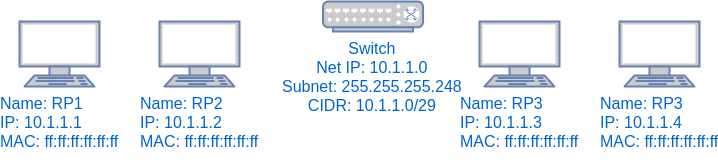
\includegraphics[scale=0.5]{switched_nw_full} 
	\caption{Skizze des LANs nach dem gegebenen Adressierungsschemas.}
	\label{switched_nw_full}
\end{figure}
Da wir pro Bankreihe vier Raspberry Pis miteinander vernetzen sollen, muss die Subnetzmaske $/29$ bzw. $255.255.255.248$ lauten. Wodurch wir die ersten 29 Bits für die Netzmaske deklarieren und die letzten 3 Bits für den Host-Anteil. Mit diesen 3 Bits können $2^3=8$ Rechner adressiert werden. Wir benötigen vier Adressen für die Raspberry Pis und zwei Standardadressen. Die erste Adresse ist die Netzadresse, die letzte Adresse ist die Broadcastadresse. Jedoch ergibt dies eine interne Fragmentierung von zwei Adressen,d.h. diese Adressen sind allokiert werden aber nicht genutzt.\\
Mit diesem Vorgehen ist das Labor wie folgt strukturiert (s. Tabelle \ref{labor_switch}):
\begin{table}[H]
\centering
\caption{Beispielkonfiguration}
\label{labor_switch}
\begin{tabular}{cccc}
\textbf{Gruppe} & \textbf{Netzwerk IP} & \textbf{Subnetzmaske} & \textbf{CIDR}\\ 
Fractals & 10.1.1.0 & 255.255.255.248 & 10.1.1.0/29  \\
1337 & 10.1.2.0 & 255.255.255.248 & 10.1.2.0/29 \\
... & & &
\end{tabular}
\end{table}
Jede Bankreihe hat eine feste IP-Range, die sie nutzen kann. Eine Kommunikation der Netzwerke über diese Segmente hinaus ist nicht möglich.

\subsubsection{On the fly Konfiguration}
Die Konfiguration der Raspberry Pis wird im Folgenden beispielhaft für ein Gerät gezeigt. Bei allen Kommandos muss das Schlüsselwort \emph{sudo} vor dem eigentlichen Befehl angeführt werden, da nicht jeder Nutzer die Netzwerkadapter konfigurieren können soll. Das Listing \ref{ip_add_addr} zeigt, wie eine \emph{IPv4}-Adresse gesetzt und aktiviert wird.
\begin{lstlisting}[style=Bash, language=Bash, label=ip_add_addr]
# via iproute2
ip addr add 10.1.1.1/29 dev eth0
ip link set eth0 up
# via net tools
ifconfig eth0 10.1.1.1 netmask 255.255.255.248 up
\end{lstlisting}
Mithilfe der Befehle \textit{ip addr show eth0} oder \textit{ifconfig eth0} kann anschließend überprüft werden, ob der Adapter die gewünschte Konfiguration hat.\\
Um zu testen, ob die Raspberry Pis sich tatsächlich erreichen können, kann das Werkzeug \emph{ping} genutzt werden. Die entsprechende Nutzung kann im Listing \ref{ping_ip} nachverfolgt werden.

\subsubsection{Persistente Umsetzung}
Da diese Umsetzung lediglich temporärer Natur ist, wird nach einem Neustart des Systems jegliche Konfiguration verworfen. Entsprechend der Aufgabenstellung soll eine persistente Lösung umgesetzt werden. Das Listing \ref{ip_persis} zeigt diese.
\begin{lstlisting}[style=Bash, language=Bash, label=ip_persis]
# /etc/network/interfaces
auto lo # automatische setzen des loopback devices (localhost)
iface lo inet loopback # setze loopback ipv4 adresse

auto eth0 # hochfahren des interfaces zur boot zeit
allow-hotplug eth0 # erlaubt kabel wechsel waehrend des betriebs
iface eth0  inet static # statische ip addr fuer interface eth0
	address 10.1.1.1 # ip addr - statisch
	netmask 255.255.255.248 # subnetzmaske
\end{lstlisting}
Wie zu sehen ist, erfolgt die Konfiguration nicht via Kommandozeilentools, sondern in einer Datei. Diese Datei befindet sich bei \emph{Raspbian} standardmäßig im Verzeichnisbaum unter \path{/etc/network/interfaces}. Die \texttt{interfaces}-Datei darf ebenfalls nur mit \emph{root}-Rechten beschrieben werden.\\
Zeile 2 und 3 befassen sich ausschließlich mit der Konfiguration des Loopback-Devices. Diese ist für die Übungsaufgabe nicht zwingend notwendig. Die Zeilen 5-9 zeigen die Konfiguration des \ac{NIC} \emph{eth0}. Zeile 5 zeigt, dass der Adapter automatisch hochgefahren werden soll. Zeile 6 kümmert sich um das Hot-Plugging. Die Zeile 7 zeigt, dass es sich um eine statische \emph{IPv4}-Adressierung des \textit{eth0}-Adapters handelt -- Stichwort \emph{inet}. Zeile 8 ist die Notation für die Adresszuweisung und Zeile 9 gibt die zu nutzende Netzwerkmaske an. Mit dieser Konfiguration kann erneut via \emph{ping} getestet werden, ob der Netzwerkstack korrekt eingerichtet wurde.\\

\textbf{Anmerkung:} In diesem Beispielprotokoll fehlen ein paar schicke Screenshots, die zeigen, dass \emph{ping} oder \emph{ifconfig} etc. korrekt funktionieren. Ich würde es sehr begrüßen, solche Screenshots zu sehen.

\section{Schluss}
Hier könnten Verweise auf Alternativen, Ausblicke und Gedanken festgehalten werden. Da ich diese nicht habe, erspare ich dies dem Leser.

\newpage
\begin{appendices}
%start of acronyms
\section{Abkürzungsverzeichnis}
\begin{acronym}[]
\acro{CIDR}{Classless Inter-Domain Routing}
\acro{DHCP}{Dynamic Host Configuration Protocol}
\acro{GNU}{GNU is Not Unix}
\acro{ICMP}{Internet Control Message Protocol}
\acro{IEEE}{Institute of Electrical and Electronics Engineers}
\acro{IETF}{Internet Engineering Task Force}
\acro{ISO}{International Standardization Organisation}
\acro{LAN}{Local Area Network}
\acro{MAC}{Media Access Control}
\acro{NDP}{Neighbor Discovery Protocol}
\acro{NIC}{Network Interface Controller}
\acro{OUI}{Organizationally Unique Identifier}
\acro{OSI}{Open Systems Interconnection}
\acro{PID}{Process Identifier}
\acro{r}{remote - entfernt}
\acro{RFC}{Request for Comments}
 \acro{SSH}{Secure Shell}
 \acro{SSH-AUTH}{Secure Shell Authentication Protocoll}
 \acro{SSH-CONN}{Secure Shell Connection Protocoll}
 \acro{SSH-ARCH}{Secure Shell Architecture Protocoll}
 \acro{SSH-TRANS}{Secure Shell Transmission Protocoll}
\acro{SoC}{System-on-a-Chip}
\acrodefplural{SoC}[SoCs]{Systems-on-a-Chip}
\acro{SLAAC}{Stateless address autoconfiguration}
\acro{tcp/ip}{Transmission Control Protocol/Internet Protocol}

\end{acronym}

%\addcontentsline{toc}{section}{}
\listoffigures

\newpage
\section{Quellen}
\bibliography{sources}
%\addcontentsline{toc}{}{}
\end{appendices}

\end{document}